%% -*- LaTeX -*-
\documentclass{report}

\usepackage{thesis}

%some other packages I found useful, comment out or remove if you do not need them
\usepackage{amsmath}
\usepackage{amssymb}
\usepackage[titletoc,toc,title]{appendix}
\usepackage{chapterbib}
\usepackage{cite}
\usepackage[pdftex]{graphicx}
\usepackage{mdframed}
\usepackage{minted}
\usepackage{multirow}
\usepackage{newunicodechar}
\usepackage{pdfcomment}
\usepackage{subfigure}
\usepackage{tabularx}
\usepackage{titlesec}
\usepackage{url}
\usepackage{xspace}

% must be loaded after hyperref
\usepackage{cleveref}

\usemintedstyle{friendly}

\newunicodechar{⇒}{\ensuremath{\Rightarrow}}
\newunicodechar{→}{\ensuremath{\rightarrow}}
\newunicodechar{λ}{\ifmmode\lambda\else\textlambda\fi}
\newunicodechar{Θ}{\ifmmode\Theta\else\textTheta\fi}
\newunicodechar{Γ}{\ifmmode\Gamma\else\textGamma\fi}
\newunicodechar{μ}{\ifmmode\mu\else\textmu\fi}
\newunicodechar{η}{\ifmmode\eta\else\texteta\fi}
\newunicodechar{Π}{\ifmmode\Pi\else\textPi\fi}
\newunicodechar{𐤄}{\ifmmode{\rotatebox[origin=c]{15}{\textphnc{e}}\hspace{-1pt}}\else{\textphnc{e}}\fi}
\newunicodechar{⊥}{\ensuremath{\bot}}
\newunicodechar{×}{\ensuremath{\times}}
\newunicodechar{⊳}{\ensuremath{\rhd}}
\newunicodechar{∩}{\ensuremath{\cap}}
\newunicodechar{∪}{\ensuremath{\cup}}
\newunicodechar{≠}{\ensuremath{\neq}}
\newunicodechar{∅}{\ensuremath{\varnothing}}
\newunicodechar{⊢}{\ensuremath{\vdash}}
\newunicodechar{△}{\ensuremath{\bigtriangleup}}
\newunicodechar{≡}{\equiv}
\newunicodechar{≢}{\not\equiv}
\newunicodechar{≤}{\ensuremath\leq}
\newunicodechar{⊕}{\oplus}
\newunicodechar{⊖}{\ominus}
\newunicodechar{⟦}{\lBrack}
\newunicodechar{⟧}{\rBrack}
\newunicodechar{∖}{\setminus}

\newcommand{\BNF}{\quad\operatorname{::=}\quad}
\newcommand{\BNFOR}{\quad\operatorname{\big{|}}\quad}
\newcommand{\CASE}[6]{\langword{case}_{#1}#2\langword{of}\INL #3 ⇒ #4 ; \INR #5 ⇒ #6}
\newcommand{\CASEm}[6]{\begin{aligned}[t]\langword{case}_{#1}#2\langword{of}&\INL #3 ⇒ #4 ;\\& \INR #5 ⇒ #6\end{aligned}}
\newcommand{\COMM}[2]{\langword{com}_{#1;#2}}
\newcommand{\cmark}{\ding{51}}%
\newcommand{\DEF}{{\quad\operatorname{\triangleq}\quad}}
\newcommand{\DEFCASE}{\quad\operatorname{\xRightarrow{△}}\quad}
\newcommand{\DOT}{\langword{.}}
\newcommand{\eg}{\textit{e.g.}\xspace}
\newcommand{\FLR}[1]{\left\lfloor{#1}\right\rfloor}
\newcommand{\FST}[1]{\langword{fst}_{#1}}
\newcommand{\FuncLang}[1][small]{$𐤄_{λ\mathrm{#1}}$\xspace}
\newcommand{\ie}{\textit{i.e.}\xspace}
\newcommand{\INL}{\langword{Inl}}
\newcommand{\inlinecode}[2][haskell]{\mintinline[breaklines]{#1}{#2}}
\newcommand{\INR}{\langword{Inr}}
\newcommand{\langword}[1]{\operatorname{\mathsf{#1}}}
\newcommand{\LOOKUP}[2]{\langword{lookup}^{#1}_{#2}}
\newcommand{\mask}{\ifmmode{\operatorname{⊳}}\else{⊳}\fi\xspace}
\newcommand{\myference}[3]{\inference[\textsc{#1}]{#2}{#3}}
\newcommand{\netstep}[2]{\xlongrightarrow{ #1 \ifthenelse{\equal{#1}{}}{}{:} #2 }}
\newcommand{\nonempty}[1]{{#1^{+}}}
\newcommand{\noop}[2]{\mathtt{noop}^{\mask #1}\!\!(#2)}
\newcommand{\PAIR}{\langword{Pair}}
\newcommand{\prcstep}[2]{\xlongrightarrow{ ⊕#1 ; ⊖#2 }}
\newcommand{\RECV}[1]{\langword{recv}_{#1}}
\newcommand{\roles}[1]{\mathtt{roles}(#1)}
\newcommand{\SEND}[1]{\langword{send}_{#1}}
\newcommand{\set}[1]{\left\{#1\right\}}
\newcommand{\SND}[1]{\langword{snd}_{#1}}
\newcommand{\step}{\operatorname{\longrightarrow}}
\newcommand{\stepname}[1]{$\mathfrak{#1}$}
\newcommand{\vdbl}{\\[8pt]}
\newcommand{\xmark}{{\large $\times$}}%

\newcommand{\ChoreographyTS}{ChoreoTS\xspace}
\newcommand{\chorLambda}{Chor$\lambda$\xspace}
\newcommand{\Chorus}{ChoRus\xspace}
\newcommand{\HasChor}{Has\-Chor\xspace}
\newcommand{\HLSCentral}{$\boldsymbol{\lambda}_{\boldsymbol{C}}$\xspace}
\newcommand{\HLSLocal}{$\boldsymbol{\lambda}_{\boldsymbol{L}}$\xspace}
\newcommand{\HLSNet}{$\boldsymbol{\lambda}_{\boldsymbol{N}}$\xspace}
\newcommand{\MultiChor}{Multi\-Chor\xspace}

\widowpenalty=1000000
\clubpenalty=1000000


\title{A New Architecture for Choreographic Programming Languages}
\author{Mako Bates}
\defensedate{June XX, 2025}
\proposal % or finalpresentation
\dissertation                             %% or \dissertation
\doctorphilosophy                      %% or \doctorphilosophy or \masterarts
\cs                                 %% this is the only speciality defined.
\graduatingIn{August}
\advisor{Joseph P. Near, Ph.D.}
\readerone{Christian Skalka, Ph.D.}
\readertwo{Yuanyuan Feng, Ph.D.}      %% Optional if MS.
\readerthree{Andrew K. Hirsch, Ph.D.}
\chair{Alice Patania, Ph.D.}
\dean{Holger Hoock, Ph.D.}  %% TODO: check title.


\begin{document}
\maketitle
\makeacceptance

\begin{abstract}
Presents both MultiChor (and possibly a distinct variant MiniChor) and a formalism "He Lambda something".
Shows how this system is more ergonomic than prior work and equally as expressive.
Expolores the theoretical minimum of choreographic programming, and implications for real use.
\end{abstract}

\begin{citationspage}
\vskip 2em
Material from this dissertation has been submitted for publication in {\it PLDI} on 06/216/2025 in the following form:\\
\vskip 2em 
\noindent Mako Bates and Shun Kashiwa and Syed Jafri and Gan Shen and Lindsey Kuper and Joseph P. Near.
	  (2025). Efficient, Portable, Census-Polymorphic Choreographic Programming. {\it PLDI25}.
\vskip 2em 
TODO: Hopefully! Hopefully, this will still be in a state of uncertainty when I defend the proposal.
Specifically, we will be in the window between rebuttal and final acceptence/rejection.

\end{citationspage}

\begin{acknowledgements}  %% Optional
Probably a shout-out to my co-authors to date.
Do I need to acknolege funding?
That's probably everything that goes here...
\end{acknowledgements}

\tableofcontents
\listoffigures
\listoftables

\mainmatter
\sloppy

%for journal format dissertation each chapter needs its own reference section, and want references to be included in global bibliography
%this is accomplished using include commands
%but, for things like the lit review (chapter 1) or an appendix, should use input so it does not get it's own references section

%if not doing a journal format dissertation you can just use input for all chapters, or put text here directly.
\chapter{Introduction and Literature Review}

\begin{quote}
Choreographic programming is a language paradigm for writing concurrent software systems of various kinds.
It's comparatively young; while some of the ideas have existed informally as far back as the 1970s,
choreographic programming as it's understood today was first formalized in~\shortcite{montesi-carbone-dfbd}.
In this chapter we describe the central concepts of choreographic programming,
its advantages and disadvantages,
and past and ongoing work to push the boundaries of the kinds of systems it can implement.
\end{quote}

\section{Introduction}

Choreographic programming (CP)
is a paradigm for implementing distributed systems in which the programmer writes one unified program, called a choreography,
that describes how the participants of the system interact
from a third-person-omniscient perspective.~\shortcite{montesi-carbone-dfbd,montesi-dissertation,montesi_book}
A choreography can be translated into to a collection of executable programs for use in the real world, one for each participant;
this process is called endpoint projection (EPP).
The CP approach has benefits both for understandability of distributed system implementations,
and for strong static guarantees about the deadlock-freedom of the resulting executable code~\cite{montesi-carbone-dfbd}.

\subsection{An illustrative example}

Consider the three programs in \Cref{fig:kvspiecewise},
which are intended to run concurrently and pass messages back and forth between each other.
The overall effect is an elementary process in which the client makes a \inlinecode{Get} or \inlinecode{Put} request to
a server (with a backup) that manages a key-value-store (KVS).
Even this simplified example takes a moment for a reader to make sense of;
one must read the three programs, infer the correspondence between messages sent and received by the three parties,
and judge for oneself if the communication protocol implemented is sensical.
One might even judge that this simple protocol has a bug:
if the request is a \inlinecode{Get}, the backup server will hang indefinitely!

\begin{figure}[tbhp]\caption{A Simple Concurrent Protocol: a key-value store with a backup server}
  \begin{mdframed}
  \begin{tabular}{c}
  \begin{minipage}{12.5cm}
    \inputminted[xleftmargin=10pt,linenos,fontsize=\scriptsize]{haskell}{figures/kvs_piecewise_client.hs.txt}
  \end{minipage} \\\\
  \begin{minipage}{12.5cm}
	  \textbf{(a)} The function to be called by the client process.
	  They pass in their \inlinecode{Request} object and send it to the server.
	  Then they receive a response from the server and return it.
  \end{minipage}\\\\
  \hline\\
  \begin{minipage}{12.5cm}
    \inputminted[xleftmargin=10pt,linenos,fontsize=\scriptsize]{haskell}{figures/kvs_piecewise_server.hs.txt}
  \end{minipage} \\\\
  \begin{minipage}{12.5cm}
  The function to be called by the primary server.
	  They pass in a reference to their mutable state, and receive a message of type \inlinecode{Request} from the client.
	  In the case of a \inlinecode{Put} request, they forward it to the backup server and check for the backup's acknowledgement.
	  In either case, they process the request against their own mutable state and send the response back to the client.
  \end{minipage}\\\\
  \hline\\
  \begin{minipage}{12.5cm}
    \inputminted[xleftmargin=10pt,linenos,fontsize=\scriptsize]{haskell}{figures/kvs_piecewise_backup.hs.txt}
  \end{minipage} \\\\
  \begin{minipage}{12.5cm}
  The function to be called by the backup server.
	  They pass in a reference to their mutable state, and receive a \inlinecode{Put} message from the primary server.
	  They process it against their mutable state and send back an acknowledgement message to indicate their success.
  \end{minipage}
  \end{tabular}
  \label{fig:kvspiecewise}
  \end{mdframed}
\end{figure}

In \Cref{sec:background} we will mention some intermediate frameworks that have historically been used to facilitate
writing large and complicated concurrent protocols,
but here we jump ahead to choreographic programming (CP).
\Cref{fig:kvspseudo} shows the same protocol as \Cref{fig:kvspiecewise}, but implemented as a choreography.
In this form there is no cognitive overhead for matching \inlinecode{send} and \inlinecode{recv} operations,
because matching pairs of them are combined into monolithic \inlinecode{comm} operations.
The entire protocol can be read at once in a sensical order.
(The order in which operations are presented in a choreography is not necessarily the order in which they will happen;
the participants are not guaranteed to all start at the same physical time, or to operate at the same speeds.)
Re-writing the example KVS system as a choreography does not immediately solve the issue
of what the backup server should do in the event of a \inlinecode{Get} request,
but it makes the problem detectable by static analysis.
In fact, the choreography in \Cref{fig:kvspseudo} cannot compile in any real CP system
because \inlinecode{"backup"}'s behavior is ambiguous.
\Cref{fig:kvsenclave} shows two variations of how to realize the KVS behavior in Haskell using our \MultiChor library.

\begin{figure}[tbhp]\caption{A Simple Choreography: a key-value store with a backup server}
  \begin{mdframed}
  \begin{tabular}{c}
  \begin{minipage}{12.5cm}
    \inputminted[xleftmargin=10pt,linenos,fontsize=\scriptsize]{haskell}{figures/kvs_pseudo.hs.txt}
  \end{minipage} \\\\
  \begin{minipage}{12.5cm}
	  A pseudo-code choreographic implementation of the protocol from \Cref{fig:kvspiecewise}.
  \end{minipage}
  \end{tabular}
  \label{fig:kvspseudo}
  \end{mdframed}
\end{figure}


\begin{figure}[tbhp]\caption{A Real Choreography: a key-value store writing using \MultiChor}
  \begin{mdframed}
  \begin{tabular}{c c}
  \begin{minipage}{8.75cm}
    \inputminted[xleftmargin=10pt,linenos,fontsize=\scriptsize]{haskell}{figures/kvsenclave_a.hs.txt}
  \end{minipage}
  &
  \begin{minipage}{3.75cm}
    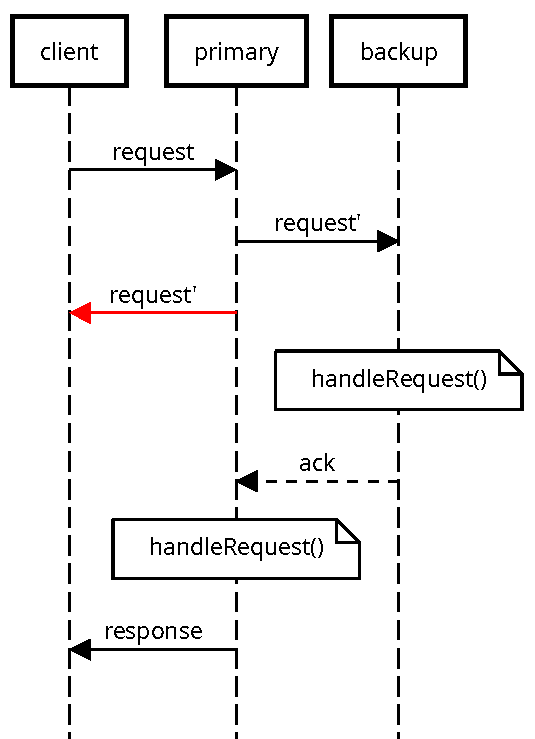
\includegraphics[width=4cm]{figures/seq2.pdf}
  \end{minipage} \\\\
  \multicolumn{2}{c}{\begin{minipage}{12.5cm}
  A key-value store with a backup server, written in \MultiChor.
           The backup server sends an acknowledgement message \textsf{ack} to the primary server
           if and only if \inlinecode{request} is a \inlinecode{Put}.
           The \inlinecode{broadcast} operator (line 19) ensures KoC
           so that the primary and backup servers are guaranteed to use the same case of \inlinecode{handleBackup},
           but it results in redundant communication (shown in red in the sequence diagram).
  \end{minipage}}\\\\
  \hline\\
  \begin{minipage}{8.75cm}
    \inputminted[xleftmargin=10pt,linenos,fontsize=\scriptsize]{haskell}{figures/kvsenclave_b.hs.txt}
  \end{minipage}
  &
  \begin{minipage}{3.75cm}
     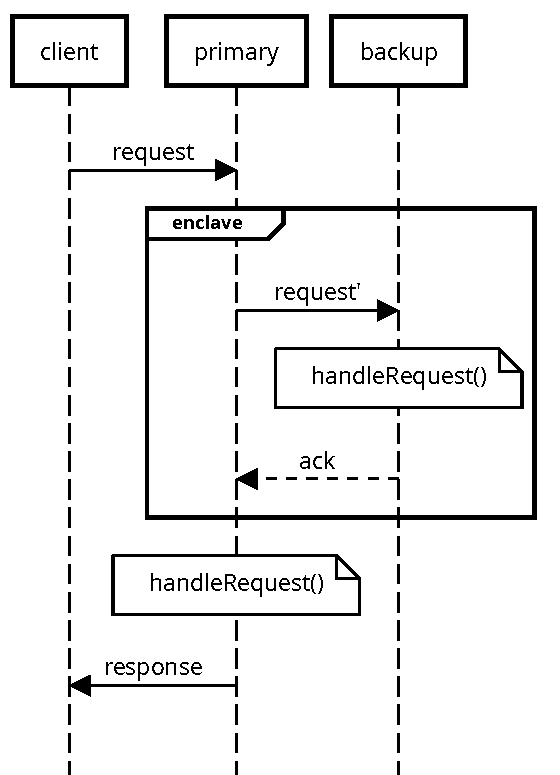
\includegraphics[width=4cm]{figures/seq3.pdf}
  \end{minipage} \\\\
  \multicolumn{2}{c}{\begin{minipage}{12.5cm}
  In this variation, the \inlinecode{enclave} operator eliminates the redundant communication.
           The enclaved sub-choreography is indicated by a box in the sequence diagram.
           On line~2, \inlinecode{@@ nobody} is \MultiChor idiom explained in \Cref{sec:membership}.
  \end{minipage}}
  \end{tabular}
  \label{fig:kvsenclave}
    %%\Description{In the top section, twenty four lines of Haskell code using the MultiChor library, with a UML sequence diagram of that program.
%%	The code defines a choreography called "kvs", and helper-functions "handleRequest" and "handleBackup".
%%	In the sequence diagram, first "client" sends "request" to "server",
%%	  then "server" sends "request-prime" to "client" and "backup",
%%	  then backup calls "handleRequest",
%%	  then backup may send "ack" to "server",
%%	  then server calls "handleRequest",
%%	  then server sends "response" to "client.
%%	The bottom sections shows changes to the code in the top section.
%%	In particular, the return type of "handleBackup" is changed to exclude "client".
%%	In the updated sequence diagram, the part of the protocol representing "handleBackup" is in a box named "enclave",
%%	  and the spurious transmission of "request-prime" from "server" to "client" is omitted.
%%	  }
  \end{mdframed}
\end{figure}


Here is a citation, \shortcite{li2021model}.

\subsection{Layout and Contributions}

The remainder of this chapter covers the history and theory of CP
and discusses some modern work relevant to the ongoing development of CP systems.
In particular, \Cref{sec:knowledge-of-choice} discusses the "Knowledge of Choice" problem,
a central difficulty in the design of CP systems,
and a number of strategies that have been used to solve it.

\Cref{sec:formalism} presents our first contribution:
a formal model of a CP system with two novel features:
\emph{multiply-located values} (MLVs)
and \emph{enclaves}.
These features combine to allow a compelling new strategy for KoC management.
In particular, all well-typed \HLSCentral choreographies are projectable and have cromulent KoC by construction.
In \Cref{sec:formalism-comparisons} we compare \HLSCentral to representative systems that use other KoC management strategies.

\Cref{sec:multichor} presents our second contribution: an implementation of the enclaves-\&-MLVs paradigm in Haskell.
The \MultiChor library is already available on Hackage, Haskell's main package management system.
\MultiChor directly implements the main concepts of \HLSCentral as a monadic eDSL in Haskell,
and combines Haskell's Hindley–Milner-based type system with a proof-witness system
to capture the requisite notion of a well-typed choreography.

Because \MultiChor is fully embedded in and interoperable with Haskell,
functional-programming patterns can be applied to the choreographic setting without further theoretical or infrastructural work.
The most important example of this, which we call "census polymorphism" is the ability to write choreographies
that are parametric over their set of participants.
This capability is novel among CP systems, and the third contribution presented in this work.
We discuss census polymorphism in greater detail in \Cref{sec:census-poly}.
\Cref{sec:future-implementation} reviews some promising future, both theoretical and at the engineering level,
that could improve \MultiChor's utility.



\section{Background}
\label{sec:background}
In this section, we give a brief overview of choreographic programming (CP).
For a comprehensive introduction to the topic, we refer the reader to~\cite{montesi_book}.

Choreographic programming is a paradigm that expresses a distributed system
as a single, global program describing the behavior and interactions of all parties.
The global view of the distributed system enables easier reasoning about the system's behavior;
for example choreographic languages can ensure \emph{deadlock freedom}~\cite{montesi-carbone-dfbd}
and choreographies can be composed modularly like normal single-threaded protocols.



\subsection{Knowledge of Choice}
\label{sec:knowledge-of-choice}

Choreographies with conditionals
(\inlinecode{if}-expressions or anything that could be used for conditional control-flow)
introduce
a challenge for endpoint projection:
\emph{some parties might not know which branch to take!}
This challenge is referred to as the \emph{knowledge of choice}  (KoC)~\cite{castagna-knowledge-of-choice} problem.
All choreographic programming languages include a strategy for KoC
that ensures that relevant parties have enough information to play their part in the program.

\subsection{Endpoint Projection}
\label{sec:endpoint-projection}
Maybe this goes before KoC; I haven't decided.

\subsection{The "Census" typing context}
\label{sec:census}
Although it is a hallmark of CP that a user may write actions for various parties in any given place in the program
without demarcations of who "control" is passing to,
it is not necessarily the case that every party that exists is eligible to take action at every place in the choreography.
Some earlier works, \eg \cite{chor-lambda}, have tracked these sets of participants in their type systems,
and used that typing context to control participation inside of function bodes.
Such a typing context plays a more active role in this present work, so we coin the term \emph{"census"}
for a typing context that controls which parties are "present" to participate in any given part of a choreography.

A party not listed in a census should will typically skip evaluating that section of the choreography.
In terms of EPP, that's done by projecting the entire clause to ⊥ or some similar marker.

\subsection{Additional Literature}
\label{sec:modern-work}

Review recent work on CP systems, including other systems that use MLVs.


\bibliographystyle{chicago}
\bibliography{refs}

\chapter{A New Core Choreographic Calculus}
\chaptermark{Formalism???} %this is the chapter heading that will show on subsequent pages
\label{sec:formalism}

\begin{quote}
Do chapters really need their own abstracts?
\end{quote}


\section{Introduction}
Plan A is to copy-paste large sections of \emph{"We Know I Know You Know"}, with revisions from the enclaves paper etc as needed.
Iff I make a new formalism, then I'll have to decide how to integrate it here. 

\section{Comparisons with other systems}
\label{sec:formalism-comparisons}
In particular, how does E\&M stack up against S\&M?
This could also just be copy-pasta, or we could expand it with something more like a proof.

A citation might help this compile? \shortcite{shen-alg-eff-cp}

\bibliographystyle{chicago}
\bibliography{refs}

\chapter{Real World Choreographic Programming}
\chaptermark{\MultiChor: Real World Choreographic Programming} %this is the chapter heading that will show on subsequent pages
\label{sec:multichor}




\section{Introduction}
In this chapter we demonstrate the practicality of conclaves-\&-MLVs choreographic programming
by presenting our implementation:
the \MultiChor Haskell library.
\MultiChor is a "just a library" CP system in the style of HasChor.
We adopt HasChor's freer-monads and handlers design pattern,
and embed the key aspects of \HLSCentral's type system as type-level constraints with a bespoke proof-witness system.
Furthermore, the flexibility of \MultiChor's API and the power of Haskell's type system together suffice to support \emph{census polymorphism},
a novel capability in CP systems.

A key innovation of \HLSCentral is that KoC is enforced entirely
by type-level management of the census.
By representing the census as a type-level variable in Haskell,
\MultiChor enables polymorphism over both the size and membership of the census,
a feature not considered in the construction of \HLSCentral.
All Haskell typing happens statically, and \MultiChor's EPP happens at runtime (like HasChor's).
This means that, like other cases of polymorphism in Haskell, location polymorphism in \MultiChor must be resolved statically.

A few other desiderata motivate our implementation:
\begin{enumerate}
    \item It should be possible to broadcast, \ie to multicast a value to the entire census,
          and to use values known to the entire census as normal (un-located) values of their type.
    \item It should be possible to know from an appropriately-written choreography's type that some
          certain party or parties are not involved, are not in its census.
          Users should be able to embed such "conclave" choreographies inside choreographies with larger,
          possibly polymorphic, censuses.
    \item The type system should be able to reason about parties'
          membership in a census or ownership-set
          with normal subset reasoning.
\end{enumerate}
The choreography in \Cref{fig:card-game} showcases the above points.
The census of the whole program appears in the type
and does not specify who the players are.
The \inlinecode{conclave} on line~16
embeds a choreography whose census is exactly the monomorphic \inlinecode{"dealer"}
and a polymorphic \inlinecode{player} (\#2).
The helper-function \inlinecode{broadcast} on line~18 functions as described in \#1.
Many examples of \#3 are automated or hidden in \MultiChor,
but on line~16 the function \inlinecode{inSuper} is applied to
\inlinecode{players :: Subset players ("dealer" : players)}
and \inlinecode{player :: Member player players}
to attest that \inlinecode{player} is present in the census.

\begin{figure*}[tbhp]
    \begin{mdframed}
  \begin{tabular}{c}
  \begin{minipage}{0.95\linewidth}
    \inputminted[xleftmargin=10pt,linenos,fontsize=\footnotesize]{haskell}{figures/census-poly-example.hs.txt}
  \end{minipage} \\\\
  \begin{minipage}{0.95\linewidth}
             This choreography is polymorphic over the number and identity of the players,
             but the party named \inlinecode{"dealer"} is an explicit member.
             The inner monad \inlinecode{CLI} that all parties have access to is a simple freer monad
             that can be handled to IO operations, or as \inlinecode{State} for testing purposes.
             The \inlinecode{newtype Card} encapsulates the modulo operation in its
             \inlinecode{Num} instance.
  \end{minipage}
  \end{tabular}
    \caption{A card game expressed as a choreography written in \MultiChor.}
    \label{fig:card-game}
    %\Description{Thirty lines of haskell code describing a choreography called "game".}
    \end{mdframed}
\end{figure*}


\section{Censuses, Conclaves, and MLVs in Haskell}
\label{sec:implementation}

\MultiChor uses the same free-monad approach as \HasChor~\cite{shen-haschor} to implement choreographic programming, EPP,
and the final interpretation to a real communication mechanism.
Also like \HasChor, \MultiChor's \inlinecode{Choreo} monad is parameterised by a \emph{local monad} in which parties' local computations can be expressed.
A \MultiChor type \inlinecode{Located ps t} is a multiply-located \inlinecode{t} owned by the parties \inlinecode{ps}.
It is possible to write \MultiChor functions that look and work like each of \HasChor's three primitive operators,
but the derived API in which users write \MultiChor choreographies contains a clear analog of only one of \HasChor's primitives.
Haskell's monadic-\inlinecode{do} notation and purity-oriented type system make \MultiChor code concise and safe
(in the sense that users are unlikely to accidentally invalidate important invariants).

As explained in \Cref{sec:formalism},
our KoC strategy requires that the correctness (well-typed-ness) of choreographies be judged in the context of a census.
\MultiChor adds the census as a type parameter of the \inlinecode{Choreo} monad.
Its kind is \inlinecode{[Symbol]},
which is to say that the census is a type-level list of parties and parties are type-level strings.
\inlinecode{Choreo} is \emph{not} an \emph{indexed} monad (that is, executing a monadic operation doesn't change the census),
but monadic operations can take choreographies with smaller censuses as arguments.

\begin{figure*}[tbhp]
  \begin{mdframed}
  \begin{tabular}{c}
  \begin{minipage}{0.95\linewidth}
    \inputminted[xleftmargin=10pt,linenos,fontsize=\footnotesize]{haskell}{figures/operators-multichor.hs.txt}
  \end{minipage} \\\\
  \begin{minipage}{0.95\linewidth}
        Of these four operators, \inlinecode{conclave} is the only one users will usually call directly;
        the other three can combine with each other (and with \inlinecode{conclave}) to make more user-friendly alternatives.
  \end{minipage}
  \end{tabular}
    \caption{
        The fundamental operators for writing expressions in \MultiChor's \inlinecode{Choreo} monad.
    }
    \label{fig:operators-multichor}
    %\Description{Four type signatures for Haskell functions using the MultiChor library.}
  \end{mdframed}
\end{figure*}

The fundamental operations of \MultiChor's \inlinecode{Choreo} monad are
\inlinecode{conclave}, \inlinecode{broadcast'}, \inlinecode{locally'}, and \inlinecode{congruently'}.
Their type signatures are given in \Cref{fig:operators-multichor}.
Like in \HasChor, these are free-monad constructors; their behavior is implemented in interpreters
that carry out EPP or implement a centralized semantics.
Three of them have their names "primed" because the un-primed versions of these names are reserved for more ergonomic derived functions.
For example, \inlinecode{locally'} takes a single argument, a computation in the local monad, and requires that the census contains
\emph{a single party}, who will execute that computation.
The un-primed \inlinecode{locally} takes an additional argument that identifies a single party from a larger census;
it uses \inlinecode{conclave} to correctly call \inlinecode{locally'}.
\inlinecode{broadcast} shares a \inlinecode{Located} value with the entire census so the unwrapped value can be used;
by combining this with \inlinecode{conclave} we can implement point-to-point or multicast communication.
From the perspective of a centralized semantics, \inlinecode{conclave} doesn't do anything at all besides run
the sub-choreography,
but EPP to a party \emph{not} in the sub-census skips the sub-choreography and just returns \inlinecode{Empty}.

\inlinecode{congruently} lets us leverage MLVs to concisely write actively-replicated computations.
In contrast to \inlinecode{locally}, the computation is performed by multiple parties
and the result is multiply-located across all of them.\footnote{
    The entire census participates in the primed version, and its result is returned naked.
    The behavior of \inlinecode{conclave} and the more fundamental rules of monadic programming
    ensure the un-primed \inlinecode{congruently} behaves correctly.
}
For the execution of these actively-replicated computations to correctly return an MLV,
all the parties must be guaranteed to be doing a pure computation on the same data.
Haskell makes it easy to enforce such a guarantee to a practical (but not unbreakable) extent.
This is why \inlinecode{congruently} does not grant access to the local monad \inlinecode{m}.
It also requires that the computation not have access to the specific identity of the computing party,
unlike \inlinecode{locally} and the similar-looking function \inlinecode{parallel} mentioned in \Cref{sec:census-poly}.
Weakening (or subverting) these restrictions would allow a user to violate \MultiChor's invariant that MLVs (\inlinecode{Located} values)
have the same value across all their owners.

It is critical to the safety of \MultiChor that the projection of a choreography to any given party will not use
any other party's \inlinecode{Located} values.
We use the same basic strategy for this as \HasChor:
\inlinecode{Located}'s constructors, \inlinecode{Wrap} and \inlinecode{Empty}, are hidden inside the core module
and afforded only by dependency injection to \inlinecode{locally} and \inlinecode{congruently}.
The specific "unwrapper" functions afforded to \inlinecode{locally} and \inlinecode{congruently}
are known to user code only by their type signatures, which have respective aliases \inlinecode{Unwrap} and \inlinecode{Unwraps}.
\inlinecode{Located}'s constructors are also used by two less-critical functions, \inlinecode{flatten} and \inlinecode{othersForget}.
These are needed for shrinking ownership sets or un-nesting \inlinecode{Located} values;
they could be written using \inlinecode{congruently},
but by implementing them in the core module where they can pattern-match \inlinecode{Located} values we are able to make them not-monadic,
and so more convenient.


\section{Membership Constraints \& Proof Witnesses}
\label{sec:membership}

It is not trivial for Haskell's type-checker (a component of GHC, the compiler) to judge if
a particular participant owns a multiply-located value or is present in a particular census
when the party or the set are polymorphic.
Declaring membership and subset relations as class constraints can work in some situations,
but this strategy has serious limitations which we find unacceptable.
For example, a rule as obvious as
$(p \in ps_1 \land ps1 \subseteq ps_2) \to p \in ps_2$,
represented in Haskell as
\inlinecode{instance ( IsMember p ps1, IsSubset ps1 ps2) => IsMember p ps2},
would be impossible to use because the compiler has no way of guessing which set \inlinecode{ps1}
it should be checking \inlinecode{p}'s membership in.
(Even if it could \emph{guess}, it wouldn't backtrack and try a different guess when its first try didn't work).

To work around such limitations, \MultiChor uses a strategy of \emph{proof witnesses}
like those described by \cite{noonanGDP}.
These are light-weight runtime values with specially crafted types,
such that the existence of a value of the given type guarantees the truth of some logical assertion.
We do not actually use the \inlinecode{gdp}\footnote{
    "Ghosts of Departed Proofs"~\cite{gdp_hackage}
} package; we found that writing our own purpose-specific system had a few advantages.
First, we were able to write everything we needed without hand-waving any foundations as \inlinecode{axiom}s.
Second, pattern matching against the constructors of \inlinecode{Member l ls} suffices to convince GHC that \inlinecode{ls} is not empty,
which is sometimes useful.
Finally, the implicit paradigm of "memberships as indices \& subsets as functions" was qualitatively easier to work with
when we were building the census-polymorphism tools described in \Cref{sec:census-poly}.

\Cref{fig:proof_witnesses} shows the implementation of this system and some of its idioms.
In \MultiChor, locations are identified by type-level strings, uninhabited types with "kind" \inlinecode{Symbol}.
A values of type \inlinecode{Member p ps} can be used both
as proof that \inlinecode{p} is eligible to take some action (because of their membership in \inlinecode{ps})
and as a term-level identifier for the party \inlinecode{p}.
The actual form of a value of type \inlinecode{Member p ps}
is equivalent to an index in the type-level list \inlinecode{ps} at which \inlinecode{p} appears.
Subset relations are expressed and used similarly:
A value of type \inlinecode{Subset ps qs} has the underlying form of a function
from \inlinecode{Member p ps} to \inlinecode{Member p qs},
\emph{universally quantified over \inlinecode{p}}.
Because these logical structures can be built from scratch inside Haskell's type system,
all of the machinery we use to do so can safely be exposed to end-users so that they can write their own proofs, as needed, inside choreographies.
For example, a user could import the types and functions shown in \Cref{fig:proof_witnesses} to write
\begin{minted}[xleftmargin=30pt,fontsize=\small]{haskell}
-- | Cons an element to the superset in a `Subset` value.
consSuper :: Subset xs ys -> Subset xs (y ': ys)
consSuper sxy = transitive sxy (Subset Later)
\end{minted}
By far the most common such manipulation we used in our case studies was
building "lists" (\inlinecode{Subset} values) out of constituent \inlinecode{Member} items
using the pattern \inlinecode{p @@ q @@ nobody} (read as \emph{"\inlinecode{p} and \inlinecode{q} and nobody else"}),
which makes a \inlinecode{Subset '[p, q] ps} out of a \inlinecode{Member p ps} and a \inlinecode{Member q ps}.

\begin{figure*}[tbhp]
  \begin{mdframed}
  \begin{tabular}{c}
  \begin{minipage}{0.95\linewidth}
    \inputminted[xleftmargin=10pt,linenos,fontsize=\footnotesize]{haskell}{figures/proof_witnesses.hs.txt}
  \end{minipage} \\\\
  \begin{minipage}{0.95\linewidth}
	  The proof witnesses are values of type \inlinecode{Member} or \inlinecode{Subset}.
	  \inlinecode{Member p ps} (line~5) is a generic algebraic data type who's constructors
	  can only be called when \inlinecode{p} actually is a member of \inlinecode{ps}.
	  \inlinecode{Subset ps qs} (line~9) values are isomorphic to functions from membership-in-\inlinecode{ps}
	  to membership-in-\inlinecode{qs}.
	  (Haskell's \inlinecode{newtype} types are intermediate between data structures and type-aliases.
	  To access the function form of a \inlinecode{Subset} one calls \inlinecode{inSuper} on it.
	  This pattern avoids impredicative typing errors.)
	  Lines~12--20 show examples of how proof witnesses can be made and combined,
	  in particular the polymorphic value \inlinecode{nobody} (line~17)
	  and the infix operator \inlinecode{@@} (line~19).
  \end{minipage}
  \end{tabular}
    \caption{
        \MultiChor's proof witness system for membership and subset constraints.
    }
    \label{fig:proof_witnesses}
  \end{mdframed}
\end{figure*}


\section{Census Polymorphism}
\label{sec:census-poly}

So far, the example choreographies we have discussed have had fixed numbers of participants.
In all prior CP systems this has been a syntactic constraint\footnote{
	\cite{cp_practice_cruz_filipe_montesi} describes an extension to Procedural Choreographies (PC)
	to allow lists of processes as arguments to procedures;
	although PC has not been implemented, the extended version would clearly be an exception to the above statement.
	}:
even systems that allow polymorphism over the identities of participants require the participants' "roles" to be explicitly defined in-context.
This is a serious limitation for writing choreographic software;
modern concurrent systems often use dozens to thousands of participants
and are defined parametrically over their number of participants~\cite{bigConcurrent1, corrigan2017prio, bigConcurrent3, bigConcurrent4, dprio2023}.
We assert that such parametric protocol declarations are a required feature for CP to find mainstream use;
our systems provide it in the form of \emph{census polymorphism}.

By "census polymorphism", we mean that a choreographic expression is polymorphic over its census type-variable,
including not just the specific identities listed but also the quantity.\footnote{
    In principle, one can split hairs between census polymorphism and similar polymorphism over other sets of parties, \eg ownership sets.
    We have not found such distinctions to be useful for describing system capabilities,
    but they can be relevant when talking about the type of a given expression.
}
Naïvely, this is trivial; any \MultiChor expression can easily be written with a type variable as its census
and the relevant parties (whose exact identities can also be polymorphic) can be guaranteed to be present by taking
membership proofs as arguments.
However, this approach has a limitation: Since the number of type variables of a choreography must be fixed
and there is no way to \emph{explicitly list} a variable number of parties,
it follows that there may be parties in the census who are not identified by the proof arguments.
Such un-enumerated parties will receive any broadcasts and participate in any active replication that applies to the whole census,
but there's no way to specify them as the senders of messages, nor is there any way to specify that they should receive a message
except by broadcasting it.
For this reason, when we speak of "census polymorphism",
we mean \emph{useful} polymorphism that lets an unspecified quantity of parties actively participate in the choreography.
For example one might wish to write a \inlinecode{gather} operation
in which a polymorphic list of participants each send a computed value to a common recipient who aggregates them.
\Cref{fig:census-poly-example} shows an example \MultiChor choreography for a key-value store with a polymorphic list of backup servers.
In \Cref{sec:mpc} we implement the GMW protocol~\cite{goldreich2019play}, a foundational protocol in multi-party cryptography.
In earlier CP systems it would have been necessary to hard-code the number of participants when writing such choreographies;
Census polymorphism is precisely the absence of such a restriction.
Census polymorphism is achieved in \MultiChor library by type-level programming in modern Haskell.

\begin{figure*}[tbhp]
  \begin{mdframed}
  \begin{tabular}{c}
  \begin{minipage}{0.95\linewidth}
    \inputminted[xleftmargin=10pt,linenos,fontsize=\footnotesize]{haskell}{figures/kvs_poly.hs.txt}
  \end{minipage} \\\\
  \begin{minipage}{0.95\linewidth}
        The main action happens in \inlinecode{handleRequest},
        a choreography involving only the servers which is called via \inlinecode{conclave} on line~27.
        \inlinecode{handleRequest}'s census explicitly includes the primary server, but is polymorphic over the list of backup servers.
        The primary server broadcasts the request (line~7); the backups will update their state and report their health
        only for a \inlinecode{Put} request.
        On lines~8--10 the backups call the local IO function \inlinecode{handlePut} in \inlinecode{parallel} using their individual state references;
        \inlinecode{oks} is therefore a \inlinecode{Faceted backups '[] Response}.
        (The extra \inlinecode{'[]} denotes that no party yet knows all of the \inlinecode{oks}.)
        \inlinecode{gather} (line~11) communicates all the \inlinecode{oks} to the primary server
        where they're stored as a \inlinecode{Quire backups Response}.
        If all the backups are ok, then the primary server also handles the request (line~14).
  \end{minipage}
  \end{tabular}
    \caption{
        A key-value store choreography with an unspecified number of backup servers.
    }
    \label{fig:census-poly-example}
    %\Description{23 lines of Haskell code using MultiChor defining a new version of "kvs" that is parametric over the number of backup servers.}
  \end{mdframed}
\end{figure*}

\subsection{Loops, Facets, and Quires}
\label{sec:census-poly-requirements}

The first thing that is necessary is a way to loop over a polymorphic list of parties.
Census polymorphism as discussed in this work is \emph{static},
\ie, while one can write choreographies and choreographic functions that are census-polymorphic,
it is always possible in principal to unroll the top-level choreography
(that actually gets compiled)
into a monomorphic form before you actually run anything.
In \Cref{sec:census-poly-haskell} we discuss \MultiChor's \inlinecode{sequenceP},
a runtime loop over statically-defined type level lists.

Less flexible options would still be viable.
The most recent versions of ChoRus and ChoreoTS lack constructs analogous to \inlinecode{sequenceP},
and instead offer the pair of functions \inlinecode[rust]{fanOut} and \inlinecode[rust]{fanIn}\cite{batesenclaves}.
These are both "for loops" over parties;
\inlinecode[rust]{fanOut}'s return type is a heterogeneous structure of the returned values for each looped-over party
(see next paragraph)
and \inlinecode[rust]{fanIn} works similarly except the owners of the aggregated data do not vary over the loop.
It's an open question whether the additional flexibility of \MultiChor's approach has any real-world use!
We also conjecture that even more restricted implementations would suffice for a majority of use-cases,
specifically by offering the three operations \inlinecode{scatter}, \inlinecode{gather}, and \inlinecode{parallel}.
\inlinecode{scatter} is multi-cast operation in which a distinct value is sent to each recipient, and \inlinecode{gather} is its dual.
\inlinecode{parallel} is exactly like \inlinecode{locally}, except a list of parties execute the local computation in parallel.
In \MultiChor, these are derived operations, and we use them frequently in our case studies.

The second thing required for useful census polymorphism is the ability to express and use divergent data known by un-enumerated parties.
We call such data structures \emph{faceted values}\footnote{
    The word "faceted" is most commonly used in reference to a cut gemstone,
    but analogy to the facets of polyhedral playing dice might be more on-the-nose.
}.
(They're basically the same as the faceted values introduced in \cite{austin2012},
except their public facet is always "$\bot$" and multiple parties have distinct private facets.)
Conceptually, a faceted value is similar to an MLV,
in that
it projects to an owner as a simple value and to a non-owner as a placeholder,
but different owners of a faceted value will have different values for it.
To see the need for faceted values, consider how one would express a census-polymorphic \inlinecode{gather} operation
using only a type-level \inlinecode{for}-loop:
The argument couldn't simply be a list,
because \inlinecode{Located} values with different owners have different types.
Each sender would need to generate its value to send \emph{inside} the loop body,
and the only way for the sent values to be distinct would be by using private local state accessed by \inlinecode{locally}.
This would hardly be satisfying, and the dual case of \inlinecode{scatter} would be even worse:
Any use to which the received values were to be put would also have to fit inside the body of the \inlinecode{for}-loop.
Again, one couldn't simply append the \inlinecode{scatter}ed values to a list and return it
because (in Haskell) all the values in a list must have the same type.

The dual of a faceted value is a "quire"\footnote{
    "Quire" is pronounced "choir"; it rhymes with "buyer" and means "a stack of sheets of paper, all cut to the same size".
    Each individual piece of paper is a "leaf".
},
a vector of values indexed by type-level parties.
Quires are not inherently located, but they can be located the same way as any other data structure.
For example, the return type of \inlinecode{gather} is
\inlinecode{Located recipients (Quire senders a)}.

\subsection{Census Polymorphism in \MultiChor}
\label{sec:census-poly-haskell}

We leverage the type system of modern Haskell to achieve useful census polymorphism in \MultiChor.
This behavior is implemented as a layer \textit{on top of} \MultiChor's central monad and data-types;
from a theory perspective \MultiChor gets census polymorphism "for free" because it's a Haskell library.
(Therefore, we do not bother with a separate proof of the soundness of census polymorphism.)
The \MultiChor repository contains over a dozen example choreographies, several of which use census polymorphism.
In \Cref{fig:census-poly-example} we showcase a key-value store choreography that's polymorphic over the number of backup servers.
\Cref{sec:mpc} presents a more involved census-polymorphic example.

Key to \MultiChor's strategy is Haskell's ability to express quantified type variables.
For example, a \inlinecode{Faceted} value is (underneath a little boiler-plate) a function.
Its argument is a \inlinecode{Member} proof that some party is in the list of owners,
and it returns a \inlinecode{Located} value known to the party in question.
Notably, nothing about the type, \inlinecode{Faceted ps cmn x}, indicates who the (type-level!) party indicated by the argument might be.
(The second type parameter, \inlinecode{cmn}, represents parties who know \emph{all} the contained values;
it's frequently \inlinecode{'[]}.)

\inlinecode{Faceted ps cmn x} is actually a special case of a more general type,
\inlinecode{PIndexed ps f}, where \inlinecode{f} can be any \emph{type-level function} from a party to a concrete type.
A \inlinecode{PIndexed} is like a type-indexed vector,
except that the type of the value retrieved depends on the index.
(The case where it does not depend on the index, \ie when \inlinecode{f} is \inlinecode{Const},
is precisely \inlinecode{Quire}.)
Because of its unusual \inlinecode{kind}, type classes that one would expect to apply to vectors generally do not apply to \inlinecode{PIndexed}.
What's actually needed for census polymorphism is the ability to \inlinecode{sequence} a \inlinecode{PIndexed} of choreographies.
Since \inlinecode{PIndexed} is not an instance of \inlinecode{Traversable},
we implement the needed function \inlinecode{sequenceP}, which is effectively just a \inlinecode{for}-loop
(in any monad) over type-level lists of parties.
These loops are not unrolled at compile time;
the type class \inlinecode{KnownSymbols} affords to the runtime environment sufficient knowledge of the type-level list.

\begin{figure*}[tbhp]
  \begin{mdframed}
  \begin{tabular}{c}
  \begin{minipage}{0.95\linewidth}
    \inputminted[xleftmargin=10pt,linenos,fontsize=\footnotesize]{haskell}{figures/census-poly-haskell.hs.txt}
  \end{minipage}
  \end{tabular}
    \caption{
        Type signatures for \inlinecode{sequenceP}, \inlinecode{fanOut}, and \inlinecode{scatter}.
    }
    \label{fig:census-poly-haskell}
    %\Description{Fourteen lines of Haskell code using the MulitChor library.}
  \end{mdframed}
\end{figure*}

The type-level programming necessary to use \inlinecode{sequenceP} and \inlinecode{PIndexed} directly
can involve some boilerplate.
We provide the derived functions \inlinecode{fanOut} and \inlinecode{fanIn}
which suffice for every situation studied so far.
\inlinecode{fanOut}'s argument is a choreography that results in a \inlinecode{Located} value at the party identified by the loop variable;
it aggregates these results as a \inlinecode{Faceted}.
\inlinecode{fanIn} is almost the same, except that the locations of the resulting values do not vary,
and they are aggregated in a \inlinecode{Quire} located at some list of recipients.
\Cref{fig:census-poly-haskell} shows the type signatures for \inlinecode{sequenceP}, \inlinecode{fanOut}, and \inlinecode{scatter}.
Keen readers may notice that the "\inlinecode{cmn}" parties' views of a \inlinecode{Faceted} are effectively just a \inlinecode{Quire},
and so wonder at the need for \inlinecode{fanIn}.
In fact, \inlinecode{fanIn} \emph{is} less often used than \inlinecode{fanOut},
but it's necessary for expressing choreographic loops that yield values which aren't known to the parties over whom the loop is defined.
For example, the GMW protocol, which we implement using \MultiChor in \Cref{sec:mpc}, cannot be written using only \inlinecode{fanOut}.

Modern Haskell language features, especially type-variable quantification,
enable \MultiChor's implementation of census polymorphism to be entirely type-safe and transparent to users.
This is a flexible system within which users can easily write their own novel and bespoke functions and data structures.


\section{The GMW Protocol in MultiChor}
\label{sec:mpc}

\emph{Secure multiparty computation}~\cite{evans2018pragmatic} (MPC) is a family of techniques that allow a group of parties to jointly compute an agreed-upon function of their distributed data without revealing the data or any intermediate results to the other parties. We consider an MPC protocol named Goldreich-Micali-Widgerson (GMW)~\cite{goldreich2019play} after its authors. The GMW protocol requires the function to be computed to be specified as a binary circuit, and each of the parties who participates in the protocol may provide zero or more inputs to the circuit. At the conclusion of the protocol, all participating parties learn the circuit's output.

The GMW protocol is based on two important building blocks: \emph{additive secret sharing}, a method for encrypting distributed data that still allows computing on it, and \emph{oblivious transfer} (OT)~\cite{naor2001efficient}, a building-block protocol in applied cryptography. The GMW protocol starts by asking each party to secret share its input values for the circuit. Then, the parties iteratively evaluate the gates of the circuit while keeping the intermediate values secret shared. Oblivious transfer is used to evaluate AND gates. When evaluation finishes, the parties reveal their secret shares of the output to decrypt the final result.

\begin{figure*}[tbhp]
  \begin{mdframed}
  \begin{tabular}{c}
  \begin{minipage}{0.95\linewidth}
    \inputminted[xleftmargin=10pt,linenos,fontsize=\footnotesize]{Haskell}{figures/gmw.hs.txt}
  \end{minipage} \\\\
  \begin{minipage}{0.95\linewidth}
      This choreography works for an arbitrary number of parties.
      \Cref{fig:gmw-helpers-multichor-example-a} contains the \inlinecode{secretShare} choreography to handle an INPUT;
      \Cref{fig:gmw-helpers-multichor-example-b} shows the \inlinecode{fAnd} choreography to compute the result of an AND gate,
      and the choreography \inlinecode{reveal}.
      \inlinecode{xor} is a non-choreographic fold function.
      \inlinecode{mpc} uses \inlinecode{gmw} and \inlinecode{reveal}, and prints the resulting bit at each party.
  \end{minipage}
  \end{tabular}
    \caption{A choreography for the GMW protocol.}
    \label{fig:gmw-multichor-example}
  \end{mdframed}
    %\Description{Thirty one lines of Haskell code using the MultiChor library.
%	This code defines a recursive choreographic function "gmw" and a top-level function "mpc".}
\end{figure*}

\begin{figure*}
  \begin{mdframed}
  \begin{tabular}{c}
  \begin{minipage}{0.95\linewidth}
    \inputminted[xleftmargin=10pt,linenos,fontsize=\footnotesize,firstnumber=1,firstline=1,lastline=15]{Haskell}{figures/gmw-helpers.hs.txt}
  \end{minipage} \\\\
  \begin{minipage}{0.95\linewidth}
      \inlinecode{secretShare} handles Input gates by secret sharing \inlinecode{p}'s secret value among \inlinecode{parties}.
      \inlinecode{genShares} uses \inlinecode{Quire} to map each member \inlinecode{p} in \inlinecode{ps} to a generated secret share \inlinecode{Bool}.
  \end{minipage}
  \end{tabular}
    \caption{Helper functions for the GMW protocol (1 of 2).
    }
    \label{fig:gmw-helpers-multichor-example-a}
  \end{mdframed}
    %\Description{Fifty nine lines of Haskell code using the MultiChor library.
%	This code defines functions "secretShare", "genShares", "xor", "fAnd", "ot2", and "reveal".}
\end{figure*}

\begin{figure*}
  \begin{mdframed}
  \begin{tabular}{c}
  \begin{minipage}{0.95\linewidth}
    \inputminted[xleftmargin=10pt,linenos,fontsize=\footnotesize,firstnumber=1,firstline=20]{Haskell}{figures/gmw-helpers.hs.txt}
  \end{minipage} \\\\
  \begin{minipage}{0.95\linewidth}
      \inlinecode{fANd} computes the result of an AND gate on secret-shared inputs using pairwise oblivious transfer.
	  The choreography works for an arbitrary number of parties, and leverages 1-out-of-2 OT.
      \inlinecode{ot} performs 1-out-of-2 oblivious transfer (OT) using RSA public-key encryption.
	  The choreography involves exactly two parties, \inlinecode{sender} and \inlinecode{receiver}.
      \inlinecode{encryptS} \inlinecode{decryptS} (which are omitted for brevity) use the cryptonite library for encryption and decryption.
      In \inlinecode{reveal}, all parties broadcast their shares of the value to each other, the gathered shares are \inlinecode{xor}ed
      to compute the plaintext result.
  \end{minipage}
  \end{tabular}
    \caption{Helper functions for the GMW protocol (2 of 2).
    }
    \label{fig:gmw-helpers-multichor-example-b}
  \end{mdframed}
    %\Description{Fifty nine lines of Haskell code using the MultiChor library.
%	This code defines functions "secretShare", "genShares", "xor", "fAnd", "ot2", and "reveal".}
\end{figure*}

\paragraph{Additive secret sharing}
We begin by describing additive secret sharing, a common building block in MPC protocols. A secret bit $x$ can be \emph{secret shared} by generating $n$ random \emph{shares} $s_1, \dots, s_n$ such that $x = \sum_{i=1}^n s_i$. If $n-1$ of the shares are generated uniformly and independently randomly, and the final share is chosen to satisfy the property above, then the shares can be safely distributed to the $n$ parties without revealing $x$---recovering $x$ requires access to all $n$ shares. Importantly, secret shares are \emph{additively homomorphic}---adding together shares of secrets $x$ and $y$ produces a share of $x+y$.

\MultiChor choreographies for performing secret sharing in the arithmetic field of booleans appear in
\Cref{fig:gmw-helpers-multichor-example-a,fig:gmw-helpers-multichor-example-b}. The function \inlinecode{secretShare} takes a single secret bit located at party \inlinecode{p}, generates \inlinecode{shares},
a \inlinecode{Quire} which maps each member in \inlinecode{parties} to a share,
and then uses \inlinecode{scatter} to send the assigned share to each member.
However \inlinecode{scatter} would return a \inlinecode{Faceted parties '[p] Bool} since by default it includes the sender.
The choreographic function \inlinecode{gmw} expects shares of wires to be secret,
so we must return a \inlinecode{Faceted parties '[] Bool}.
We accomplish this by deconstructing and reconstructing via \inlinecode{PIndexed},
and using \inlinecode{othersForget (First @@ nobody)}.
The resulting \inlinecode{Faceted} "bit" actually represents the differing values located at all parties;
the bits held by the parties sum up to the original secret.
\inlinecode{reveal} takes exactly such a shared value and broadcasts
all the shares so everyone can reconstruct the plain-text.

\paragraph{Oblivious transfer}
The other important building block of the GMW protocol is oblivious transfer (OT)~\cite{naor2001efficient}.
OT is a 2-party protocol between a \emph{sender} and a \emph{receiver}.
In the simplest variant (\emph{1 out of 2} OT, used in GMW), the sender inputs two secret bits $b_1$ and $b_2$,
and the receiver inputs a single secret \emph{select bit} $s$.
If $s=0$, then the receiver receives $b_1$; if $s=1$, then the receiver receives $b_2$.
Importantly, the sender does \emph{not} learn which of $b_1$ or $b_2$ has been selected,
and the receiver does \emph{not} learn the non-selected value.

Oblivious transfer is a \emph{two-party protocol}; it would be erroneous for any third-parties to be involved in the implementation.
\MultiChor's \inlinecode{Faceted} values and utilities for type-safe embedding of conclaved sub-protocols within larger censuses
make it possible to embed the use of pairwise oblivious transfer between parties in a general version of multi-party GMW.

\paragraph{Computing secret-shared AND via OT}
To compute the result of an AND gate, the parties compute \emph{pair-wise} ANDs using their respective shares of the input values,
then use the results to derive shares of the gate's output.
The \inlinecode{fAnd} choreography (\Cref{fig:gmw-helpers-multichor-example-b} lines~1--27)
takes \inlinecode{Faceted} values holding the parties' shares of the input values,
and returns a \inlinecode{Faceted} value representing each party's share of the output.
On line~10, the parties perform a \inlinecode{fanOut} to begin the pairwise computation;
the \inlinecode{fanIn} on line~12 completes the pairing,
and uses \inlinecode{conclaveTo} (line~20) to embed pairwise OTs (via \inlinecode{ot2}) in the larger set of parties.

\paragraph{The GMW protocol}
The complete GMW protocol operates as summarized earlier, by secret sharing input values and then evaluating the circuit gate-by-gate.
Our implementation as a \MultiChor choreography appears in \Cref{fig:gmw-multichor-example},
defined as a recursive function over the structure of the circuit.
The choreography returns a \inlinecode{Faceted} value, representing the secret-shared output of the circuit.
For ``input'' gates (lines~4--6), the choreography runs the secret sharing protocol in \Cref{fig:gmw-helpers-multichor-example-a}
to distribute shares of the secret value.
For XOR gates (\Cref{fig:gmw-multichor-example} lines~16--18),
the parties recursively run the GMW protocol to compute the two inputs to the gate
and then each party computes one share of the gate's output by XORing their shares of the inputs.
This approach leverages the additive homomorphism of additive secret shares.
For AND gates (lines~13--15), the parties compute shares of the gate's inputs,
then use the \inlinecode{fAnd} protocol to perform multiplication of the two inputs.
This implements the protocol as described in  Section 3.2.1 of \cite{evans2018pragmatic},
namely the \emph{Generalization to more than two parties} case.
Since additive secret shares are not multiplicatively homomorphic,
this operation leverages the oblivious transfer protocol to perform the multiplication.

Our implementation of GMW leverages \MultiChor's \inlinecode{Faceted} values
and utilities for type-safe parallel, conclaved, and pairwise choreographies to build a fully-general implementation
of the protocol that works for an arbitrary number of parties.

\bibliographystyle{chicago}
\bibliography{refs}


\bibliographystyle{chicago}
\bibliography{refs}

\appendix
\addappheadtotoc

\titleformat{\chapter}[hang] 
{\normalfont\huge\bfseries}{\chaptertitlename\ \thechapter:}{1em}{} 

\chapter{Parameters}
\label{journal:app:Params}
\begin{table}[h!]
\caption{Algorithm Parameters.}
\begin{center}
\begin{tabularx}{\textwidth}{ |X|X| }
%\begin{tabular}{|l|l|}
\hline
 {\bf Parameter Name} & {\bf Value}  \\ \hline \hline
 %\multicolumn{2}{|c|}{Evolutionary Algorithm Parameters} \\
 %\hline
 Population Size & 1000 \\
 Max Generations & 5000 \\ 
 Mutation Rate  & 0.03 \\
 \hline
\end{tabularx}
\end{center}
\vspace{-0.4cm}
\label{journal:tab:Params1}
\end{table} 



\end{document}
